\section{Geometry}
Problem set up requirements: 
\begin{itemize}
	\item{Materials seen in accelerator-driven systems}
	\item{Neutron fluxes representative of accelerator-driven systems}
	\item{Irradiation times}
\end{itemize}
%
The geometry chosen for this analysis is shown in Figures 
\ref{fig:snilb3D} and \ref{fig:snilbxy}. 
%
\begin{figure}[h]
	\centering
	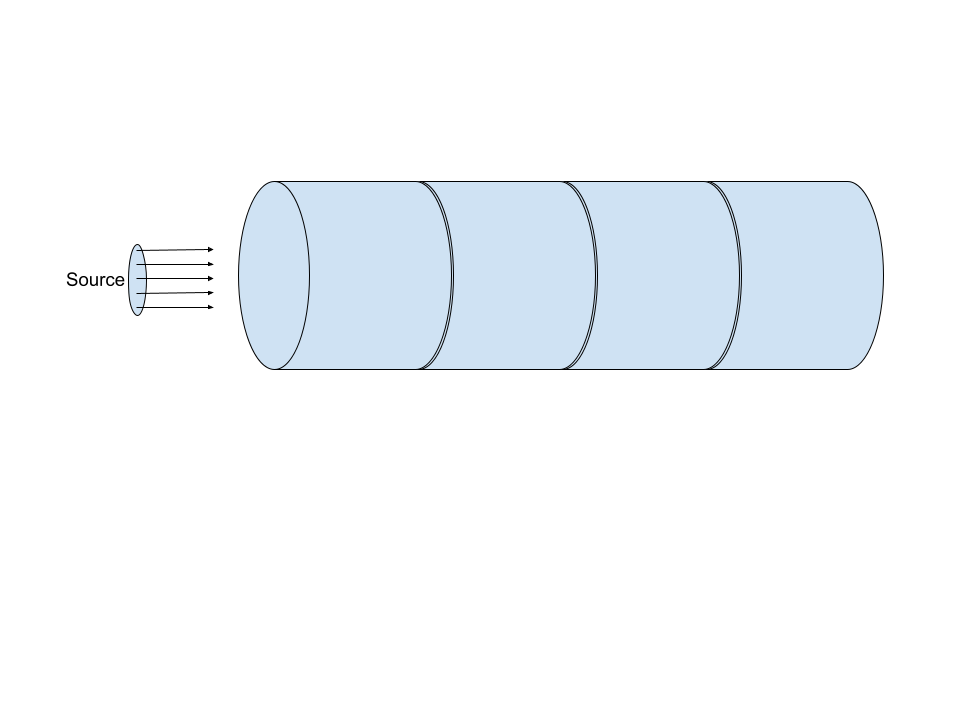
\includegraphics[scale=0.5]{figs/snilb3D_view.png}
	\caption{Overall view of geometry}
	\label{fig:snilb3D}
\end{figure}
\begin{figure}[!h]
	\centering
	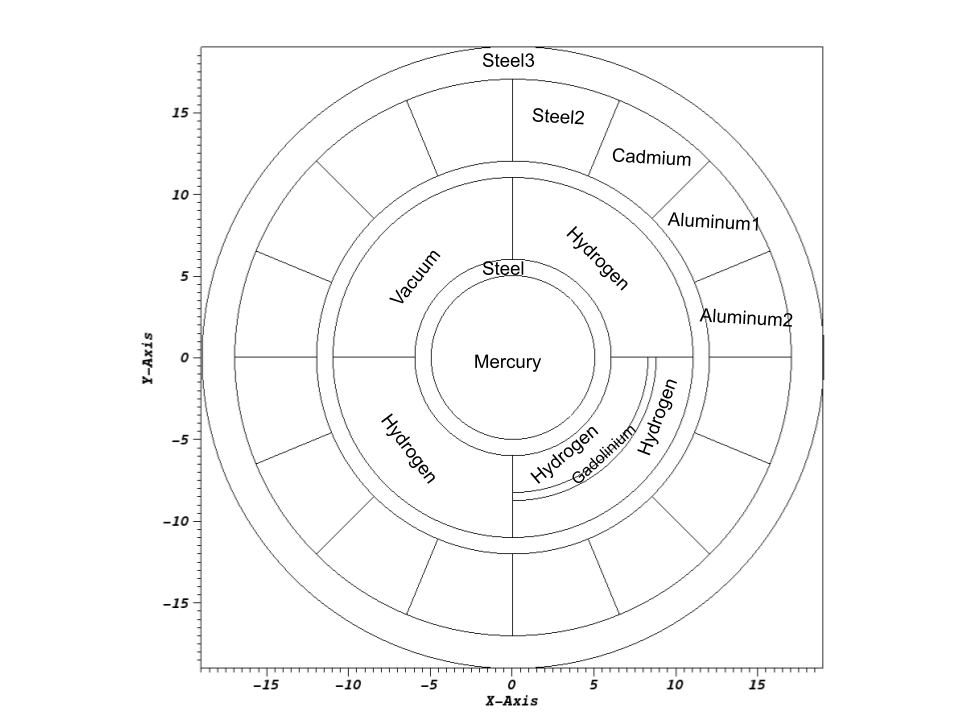
\includegraphics[scale=0.5]{figs/snilb_xy_labeled.png}
	\caption{XY cutout view of geometry}
	\label{fig:snilbxy}
\end{figure}
%
The source is a 1 GeV proton source on a disk of ratio 5 cm and 
positioned at x = -20 cm. 

%
This geometry uses materials definitions given in tables (need to add this)

\section{Workflow}
This analysis has been run so far as a cell-based workflow. 
Each of the four sections in 
Figure \ref{fig:snilb3D} has 26 volumes. 
The flux up to 20 MeV and the rnucs information is collected for each 
volume in the geometry. 
The neutron energy groups are given in Table \ref{tab:En}
\begin{table}[h]
	\caption{Neutron Enegy groups}
	\centering
		\begin{tabular}{|r|r|r|r|r|r|r}
		\cline{1-6}
		1.00E-11 & 5.00E-09 & 1.00E-08 & 1.50E-08 & 2.00E-08              & 2.50E-08              &  \\ \cline{1-6}
		3.00E-08 & 3.50E-08 & 4.20E-08 & 5.00E-08 & 5.80E-08              & 6.70E-08              &  \\ \cline{1-6}
		8.00E-08 & 1.00E-07 & 1.52E-07 & 2.51E-07 & 4.14E-07              & 6.83E-07              &  \\ \cline{1-6}
		1.13E-06 & 1.86E-06 & 3.06E-06 & 5.04E-06 & 8.32E-06              & 1.37E-05              &  \\ \cline{1-6}
		2.26E-05 & 3.73E-05 & 6.14E-05 & 1.01E-04 & 1.67E-04              & 2.75E-04              &  \\ \cline{1-6}
		4.54E-04 & 7.49E-04 & 1.23E-03 & 2.04E-03 & 2.40E-03              & 2.84E-03              &  \\ \cline{1-6}
		3.36E-03 & 5.53E-03 & 9.12E-03 & 1.50E-02 & 1.99E-02              & 2.55E-02              &  \\ \cline{1-6}
		4.09E-02 & 6.74E-02 & 1.11E-01 & 1.83E-01 & 3.02E-01              & 3.89E-01              &  \\ \cline{1-6}
		4.98E-01 & 0.639279 & 0.82085  & 1.10803  & 1.35335               & 1.73774               &  \\ \cline{1-6}
		2.2313   & 2.86505  & 3.67879  & 4.96585  & 6.065                 & 10                    &  \\ \cline{1-6}
		14.9182  & 16.9046  & 20       & 1000      & \multicolumn{1}{l|}{} & \multicolumn{1}{l|}{} &  \\ \cline{1-6}
		\end{tabular}
		\label{tab:En}
\end{table}


The total photon emission density is calculated using all fluxes and rnucs information. 
The photon emission density is also calulated using neutron flux for energy groups up to 20 MeV 
and rnucs information only for one group which includes anything above 20 MeV. 
This groups uses a neutron flux of zero. 


\section{Results}
The quantity $\eta$ is calculated using Equation \ref{eq:eta}. 
\begin{equation}\label{eq:eta}
    \eta= \sum_{h} \frac{\sum\limits_{g}^{G-1} q_{p,h}(\phi_{n,g}) + 
    q_{p,h} (Y_{n,G})}
    {q_{p,h}( \phi_{n}, Y_{n})}
\end{equation}


% MERCURY
\begin{figure}[!ht]
    \begin{subfigure}{0.5\textwidth}
        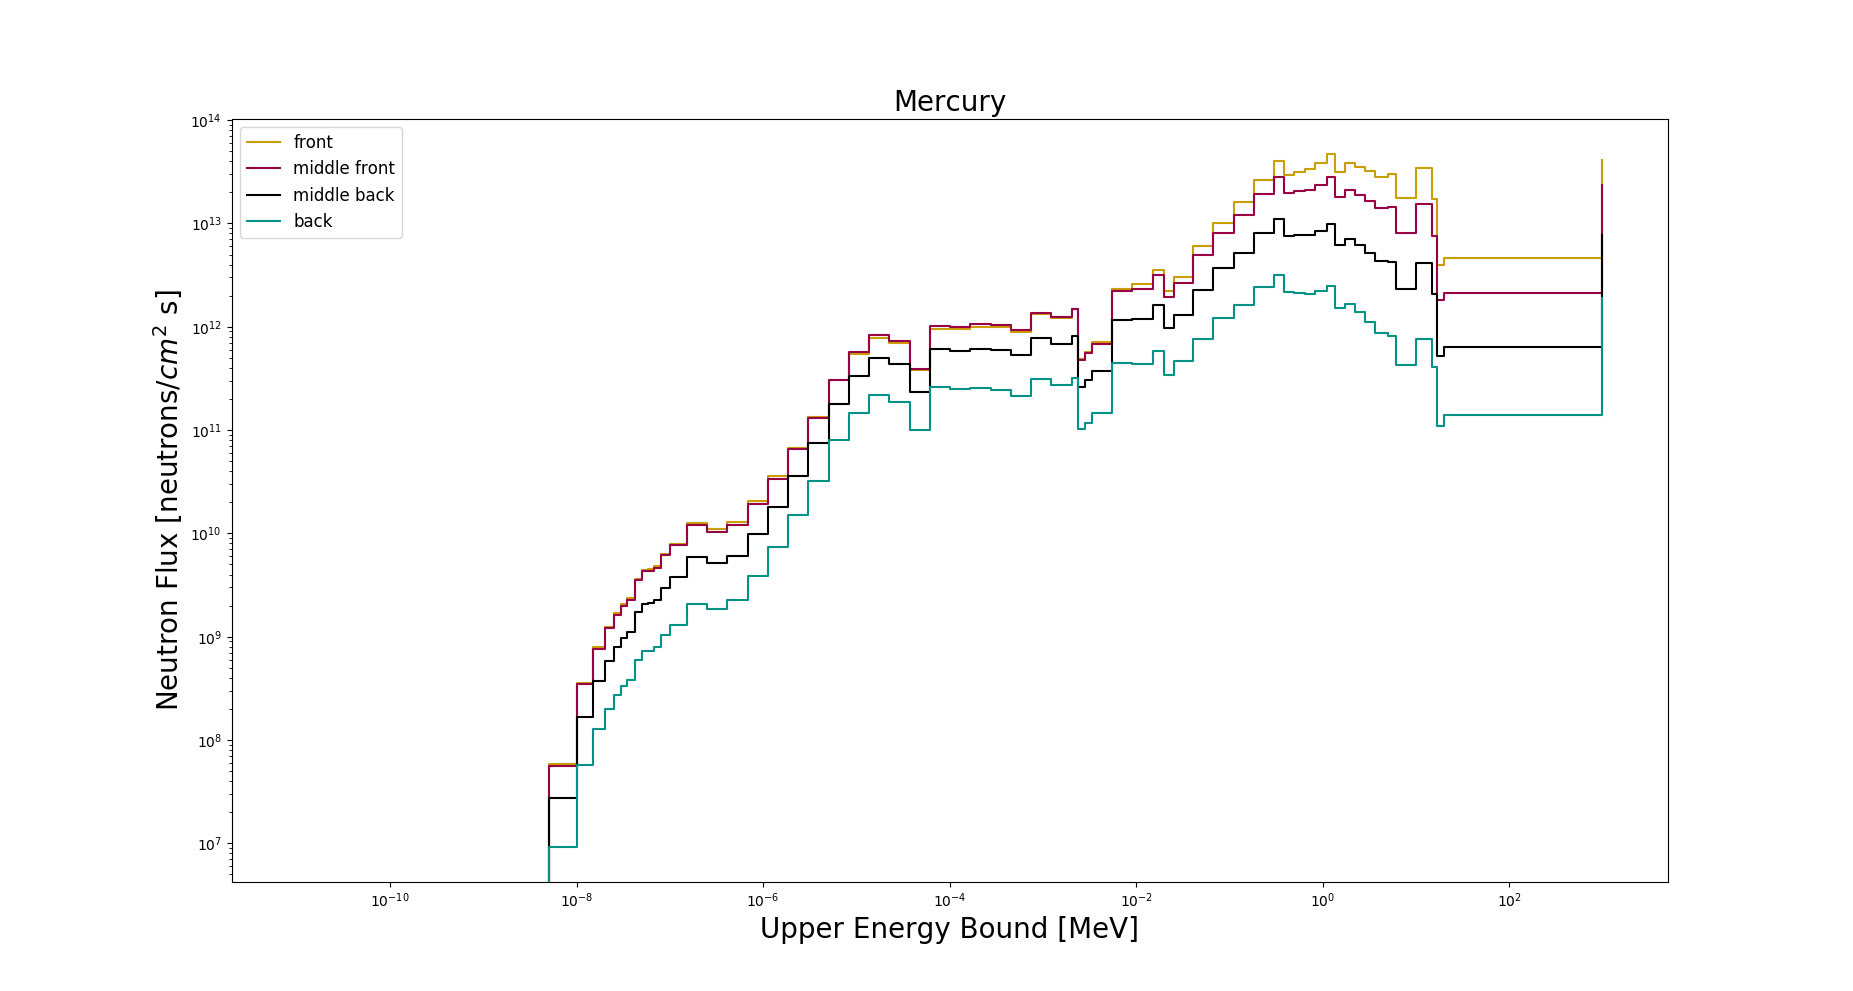
\includegraphics[scale=0.23, trim={4cm 1cm 4cm 2cm},clip]{figs/mer_flux.png}
    \end{subfigure}
    \begin{subfigure}{0.5\textwidth}
        \centering
        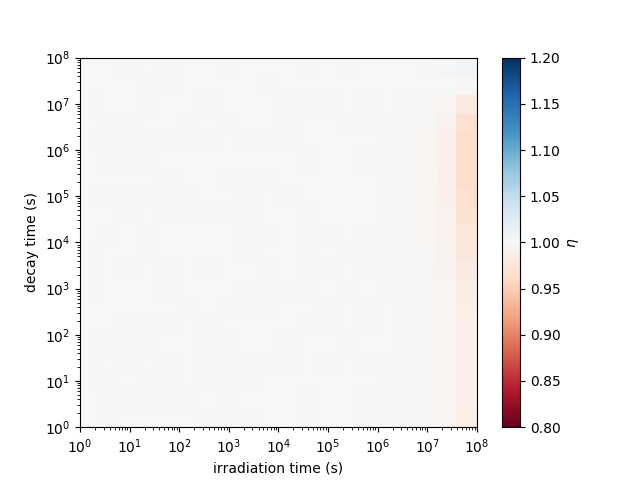
\includegraphics[scale=0.45, trim={0cm 0cm 2cm 0cm},clip]{figs/mer_front.png}
    \end{subfigure}
    \caption{Mercury}
    \label{fig:1spec_8v}
\end{figure}
% STEEL
\begin{figure}[!ht]
    \begin{subfigure}{0.5\textwidth}
        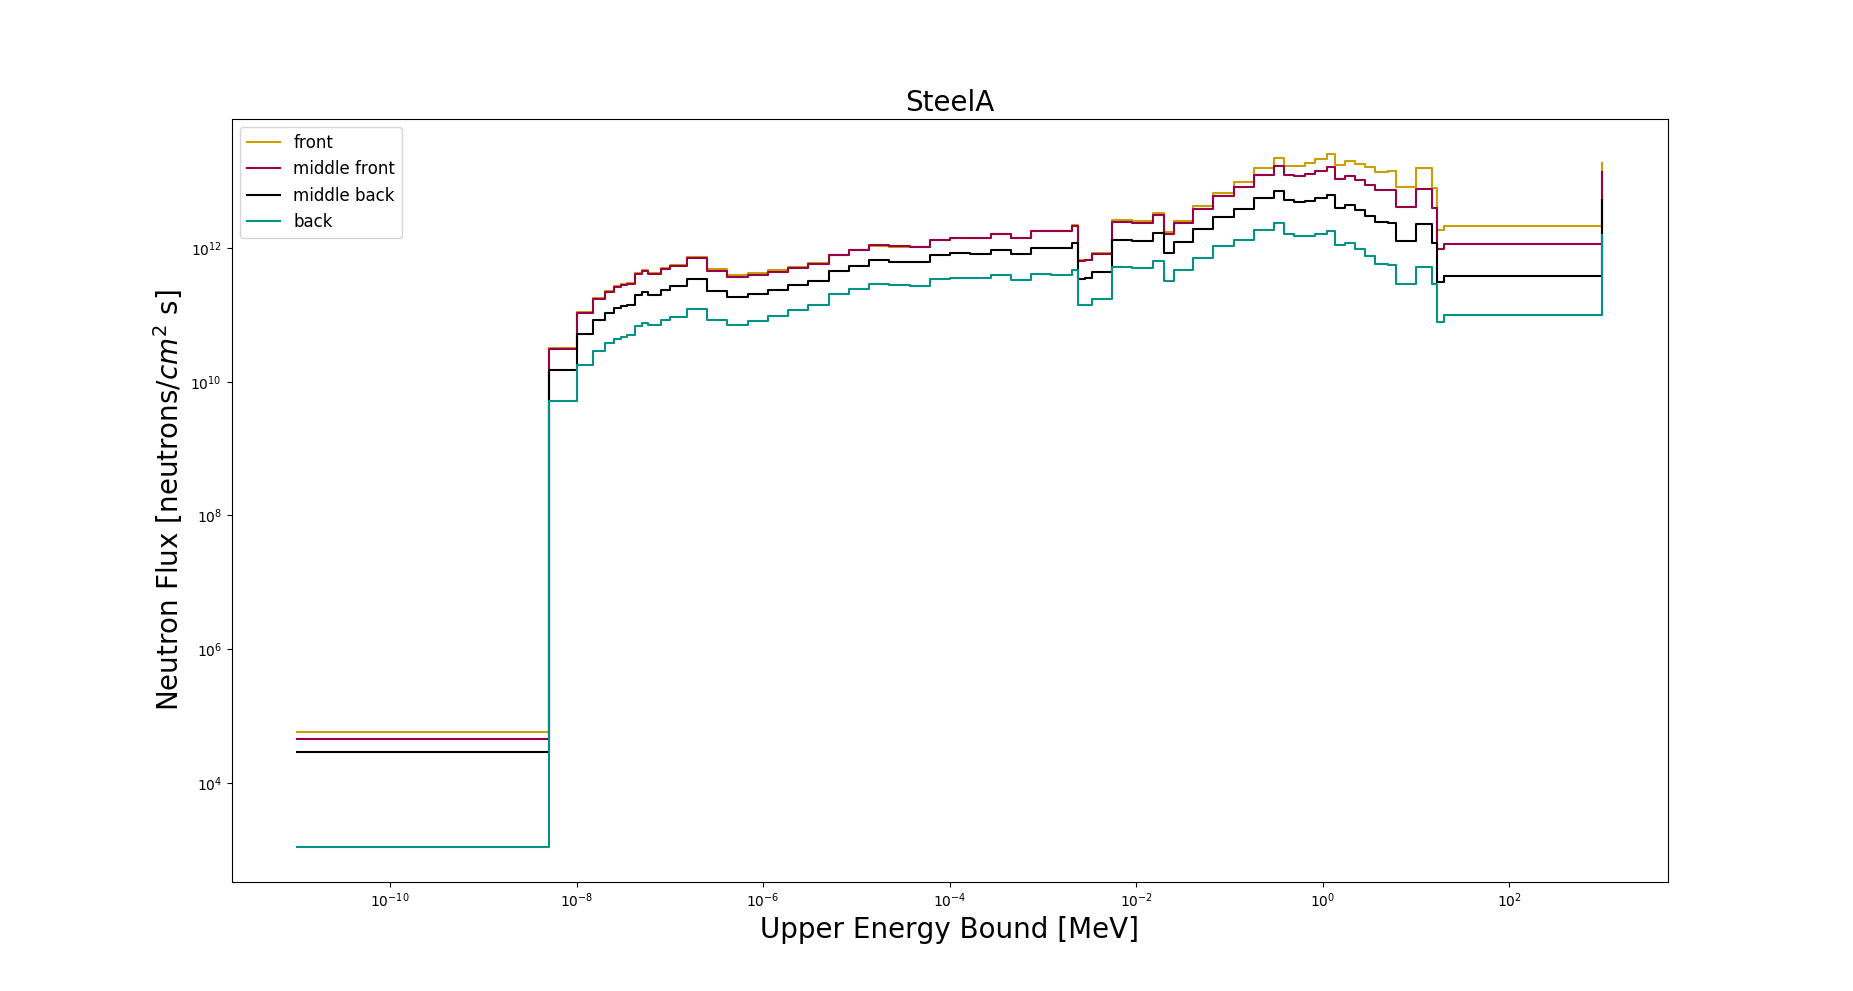
\includegraphics[scale=0.23, trim={4cm 1cm 4cm 2cm},clip]{figs/steelA_flux.png}
    \end{subfigure}
    \begin{subfigure}{0.5\textwidth}
        \centering
        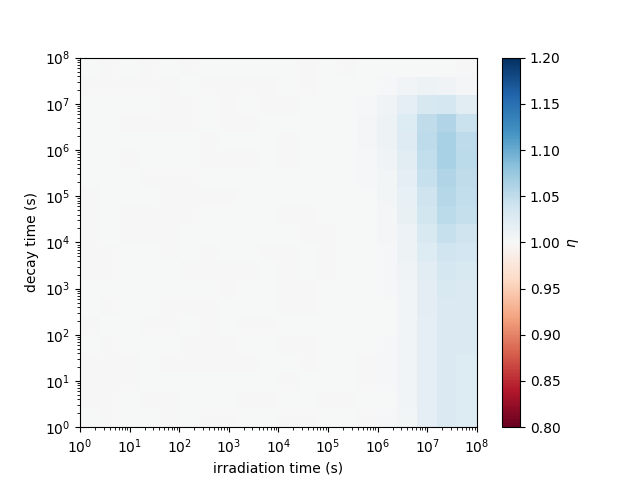
\includegraphics[scale=0.45, trim={0cm 0cm 2cm 0cm},clip]{figs/steelA_front.png}
    \end{subfigure}
    \caption{Steel}
    \label{fig:1spec_8v}
\end{figure}
% HYDROGEN1
\begin{figure}[!ht]
    \begin{subfigure}{0.5\textwidth}
        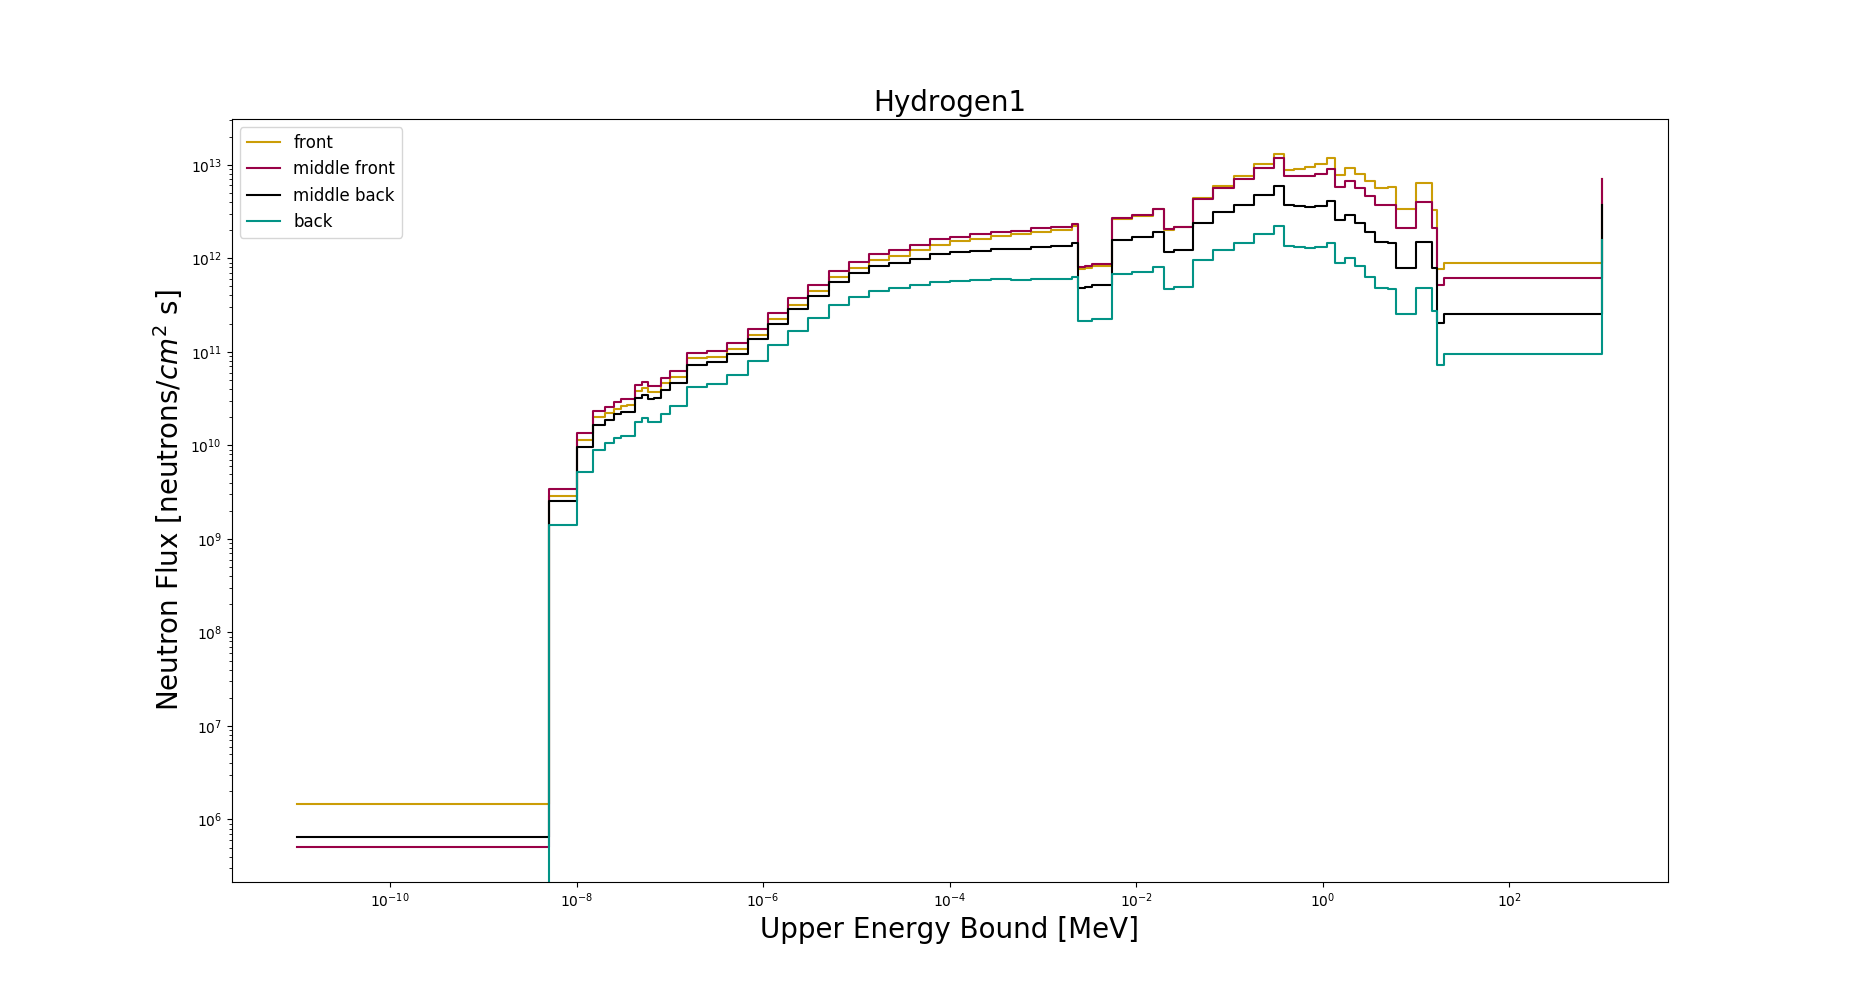
\includegraphics[scale=0.23, trim={4cm 1cm 4cm 2cm},clip]{figs/hydrogen1_flux.png}
    \end{subfigure}
    \begin{subfigure}{0.5\textwidth}
        \centering
        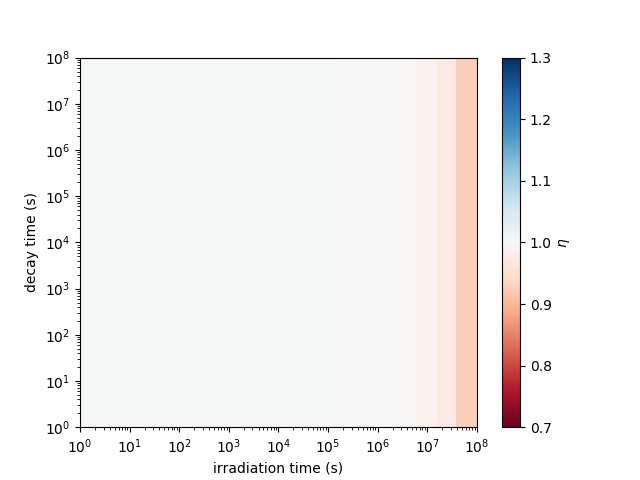
\includegraphics[scale=0.45, trim={0cm 0cm 2cm 0cm},clip]{figs/hydrogen1_front.png}
    \end{subfigure}
    \caption{Hydrogren 1 }
    \label{fig:1spec_8v}
\end{figure}
% HYDROGEN2
\begin{figure}[!ht]
    \begin{subfigure}{0.5\textwidth}
        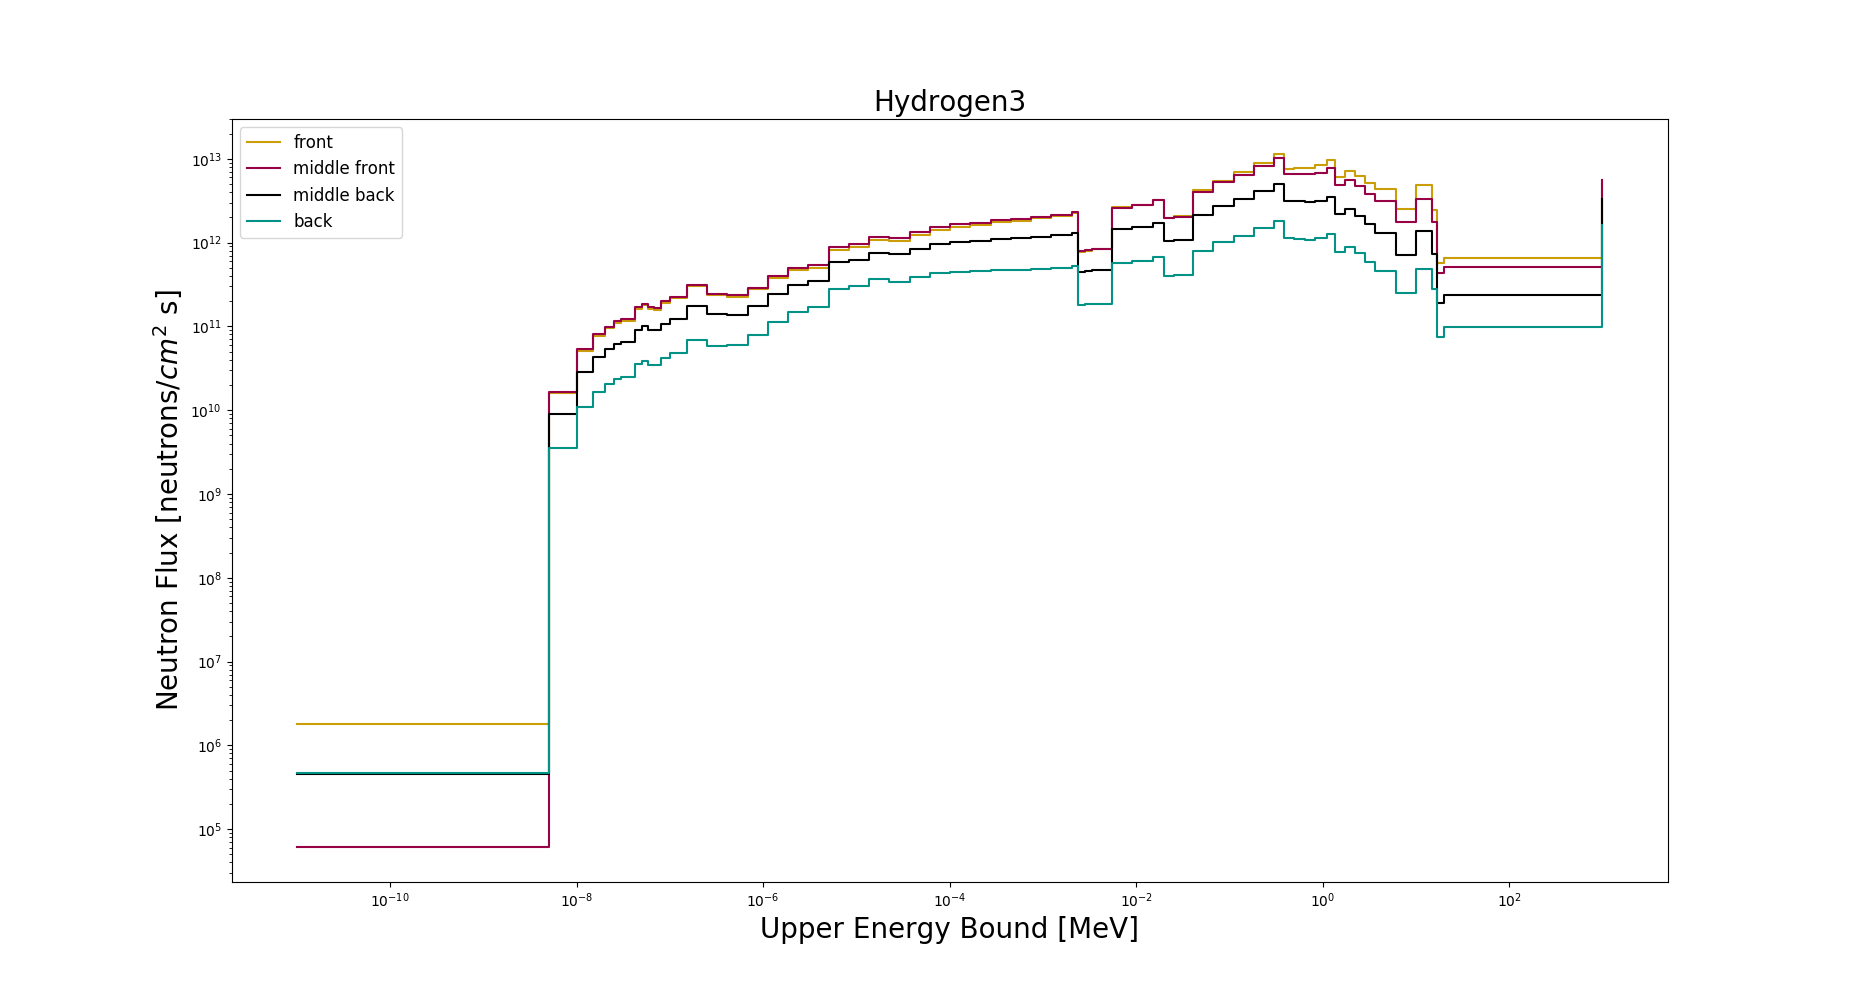
\includegraphics[scale=0.23, trim={4cm 1cm 4cm 2cm},clip]{figs/hydrogen3_flux.png}
    \end{subfigure}
    \begin{subfigure}{0.5\textwidth}
        \centering
        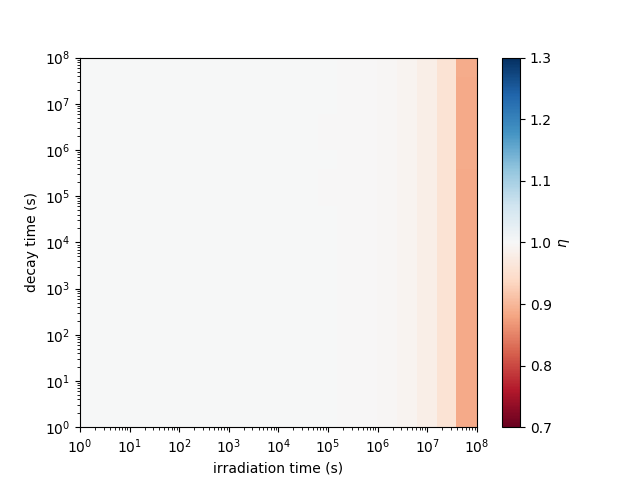
\includegraphics[scale=0.45, trim={0cm 0cm 2cm 0cm},clip]{figs/hydrogen3_front.png}
    \end{subfigure}
    \caption{Hydrogren 3 }
    \label{fig:1spec_8v}
\end{figure}
% WATER
\begin{figure}[!ht]
    \begin{subfigure}{0.5\textwidth}
        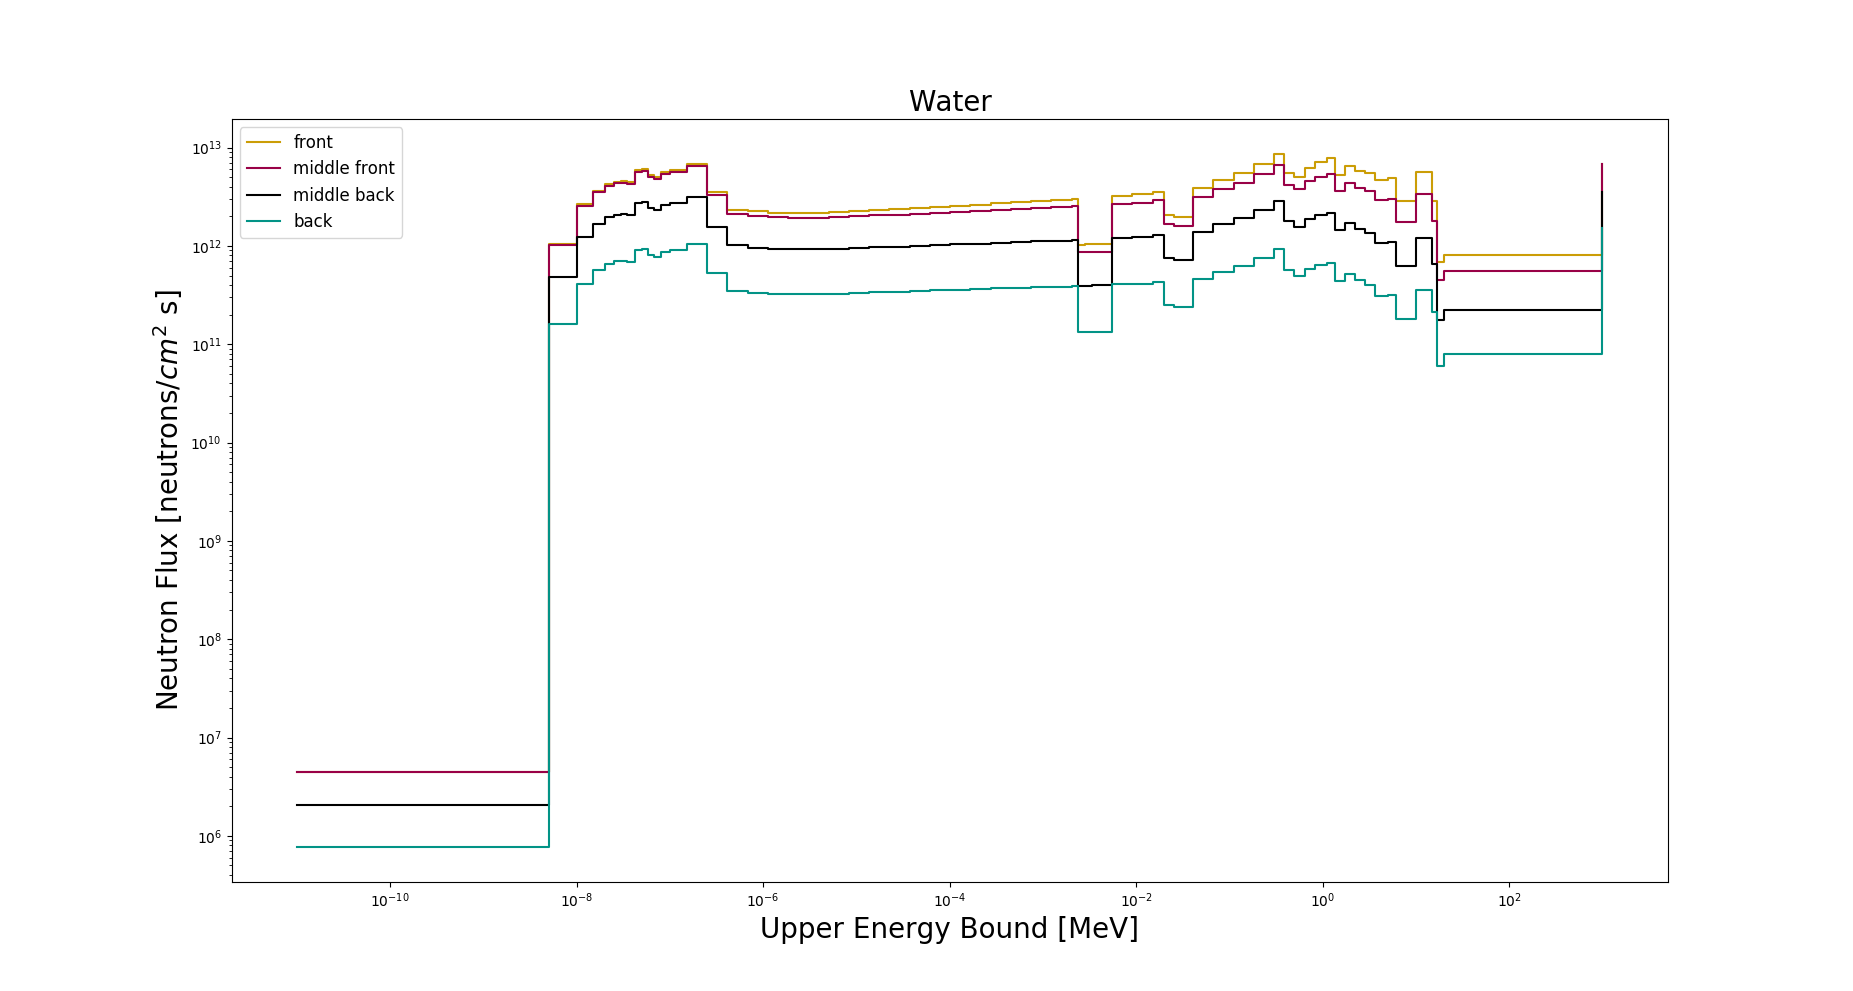
\includegraphics[scale=0.23, trim={4cm 1cm 4cm 2cm},clip]{figs/water_flux.png}
    \end{subfigure}
    \begin{subfigure}{0.5\textwidth}
        \centering
        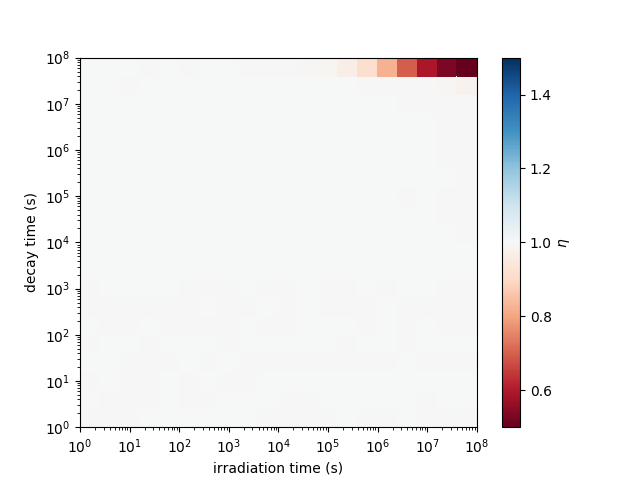
\includegraphics[scale=0.45, trim={0cm 0cm 2cm 0cm},clip]{figs/water_front.png}
    \end{subfigure}
    \caption{Hydrogren 3 }
    \label{fig:1spec_8v}
\end{figure}
% BERYLLIUM
\begin{figure}[!ht]
    \begin{subfigure}{0.5\textwidth}
        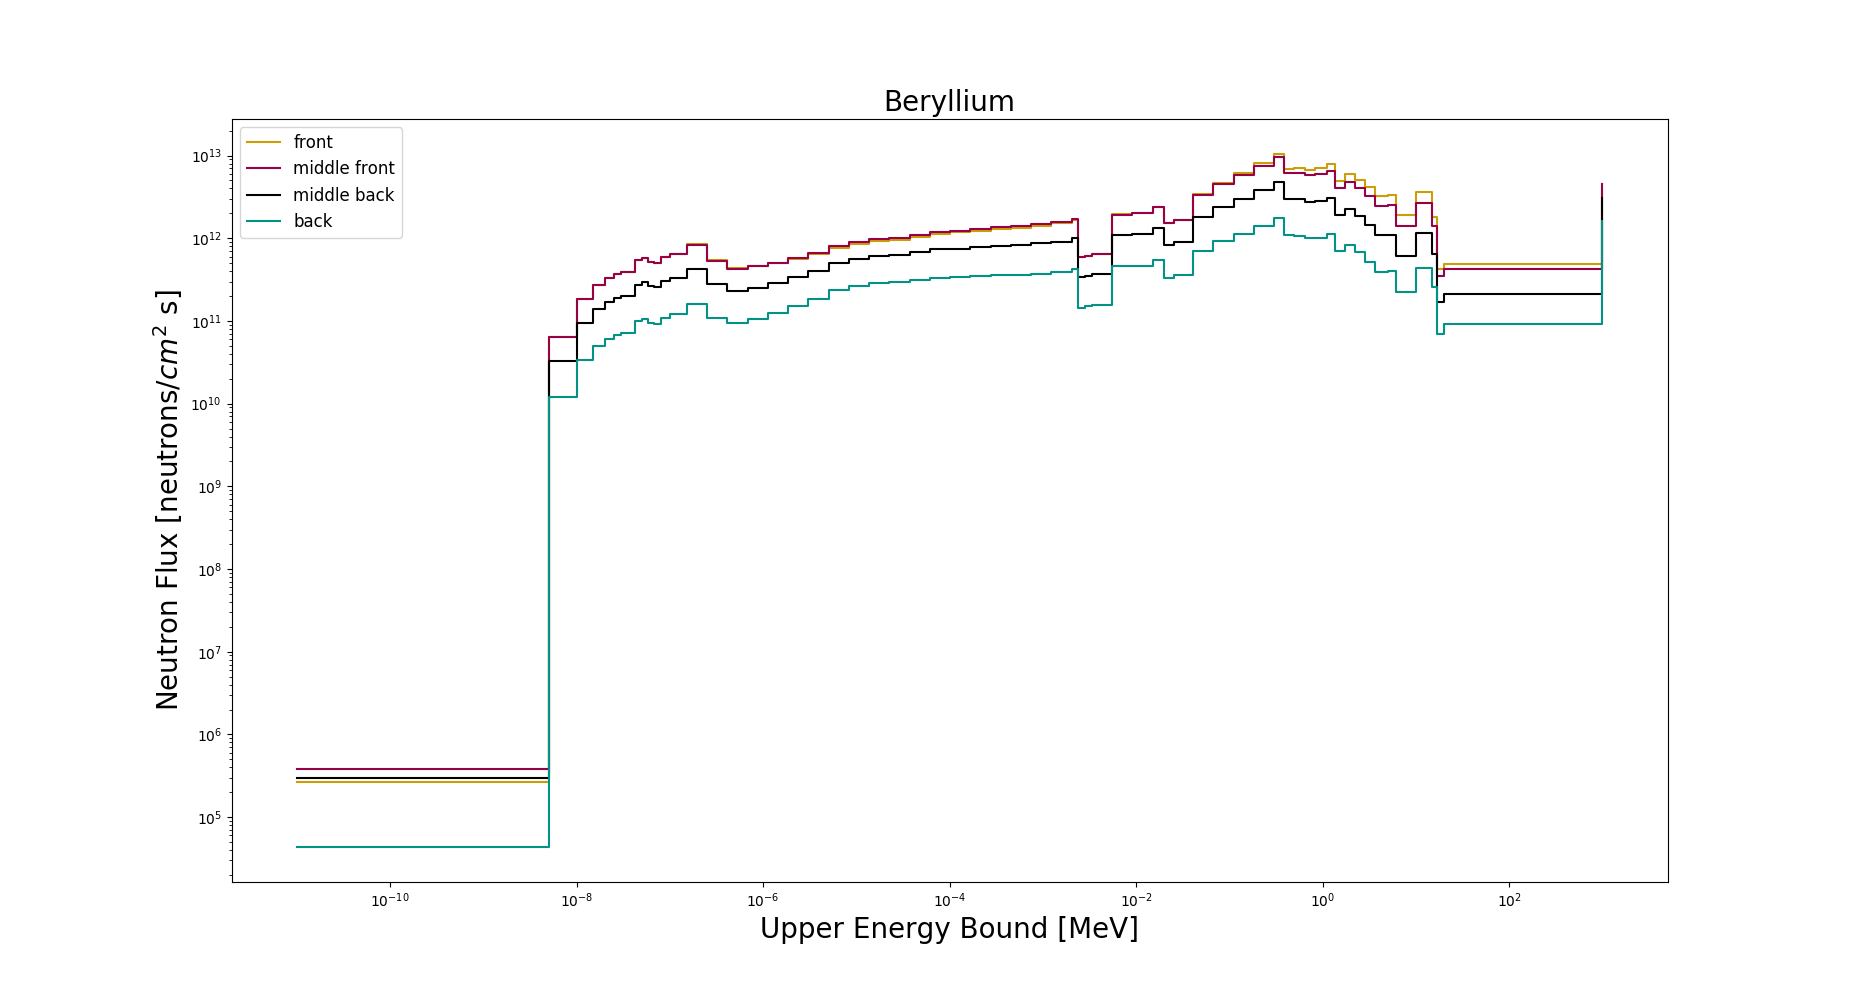
\includegraphics[scale=0.23, trim={4cm 1cm 4cm 2cm},clip]{figs/be_flux.png}
    \end{subfigure}
    \begin{subfigure}{0.5\textwidth}
        \centering
        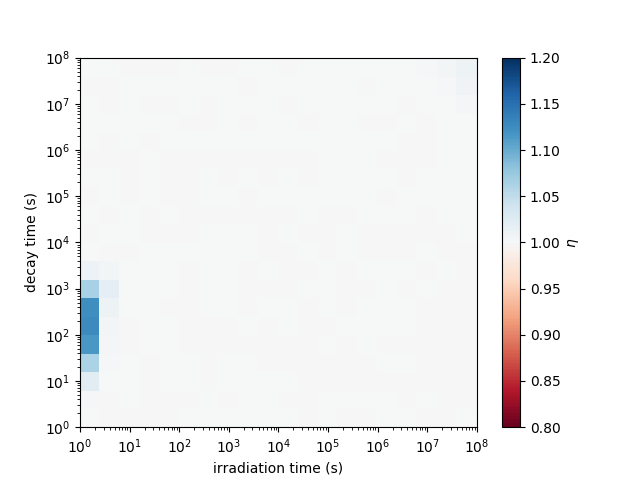
\includegraphics[scale=0.45, trim={0cm 0cm 2cm 0cm},clip]{figs/be_front.png}
    \end{subfigure}
    \caption{Beryllium }
    \label{fig:1spec_8v}
\end{figure}
% BERYLLIUM
\begin{figure}[!ht]
    \begin{subfigure}{0.5\textwidth}
        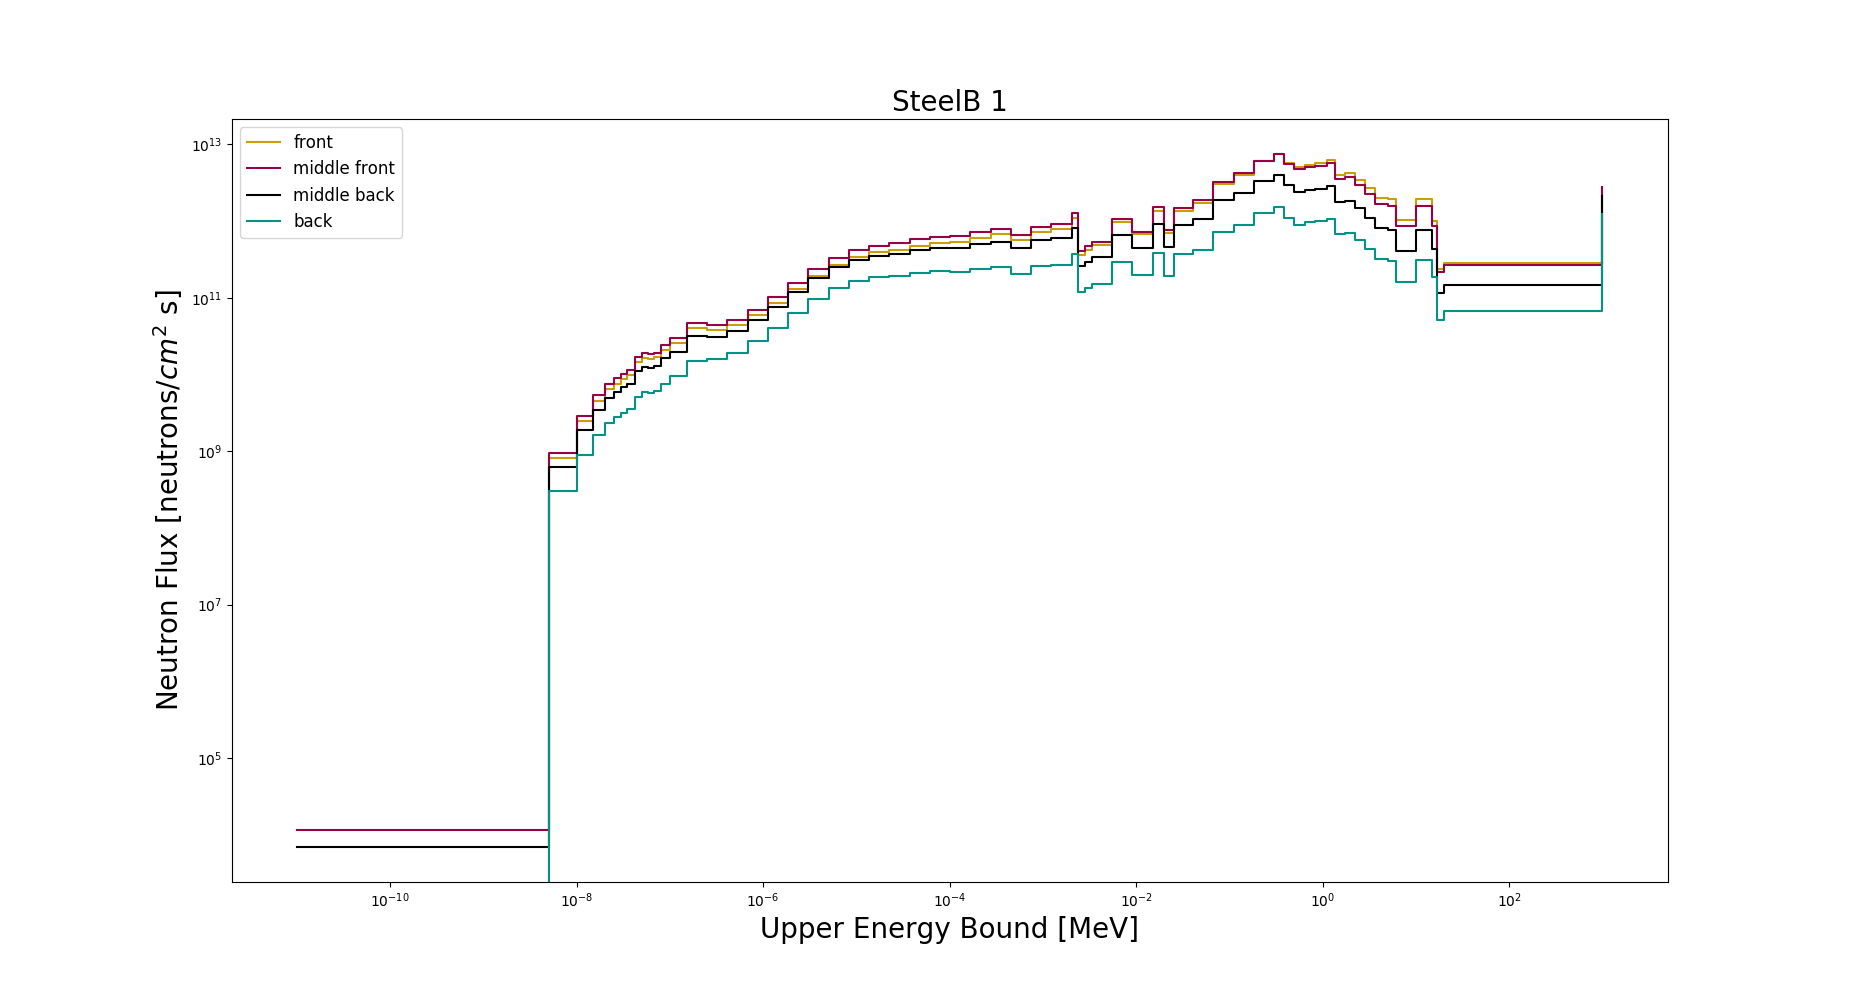
\includegraphics[scale=0.23, trim={4cm 1cm 4cm 2cm},clip]{figs/steelB1_flux.png}
    \end{subfigure}
    \begin{subfigure}{0.5\textwidth}
        \centering
        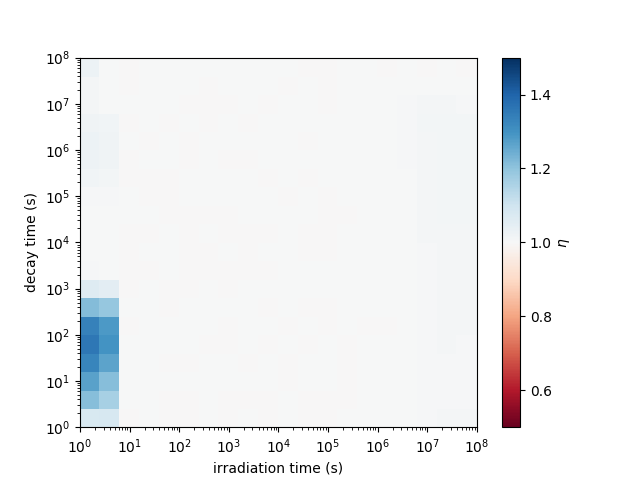
\includegraphics[scale=0.45, trim={0cm 0cm 2cm 0cm},clip]{figs/steelB1_front.png}
    \end{subfigure}
    \caption{Steel B1 (outside of H mod ) }
    \label{fig:1spec_8v}
\end{figure}